\section{Estructura}
En esta sección se detalla la estructura de todos los componentes de software de OpenGlove, los cuales son: el software de control Arduino, la API de bajo nivel C\#, las APIs de alto nivel  y la aplicación de configuración.





\subsection{Software de control Arduino}
La estructura del sofware de control Arduino corresponde a la desarrollada por \cite{tesis-cerda-rodrigo}, esta estructura se mantiene para este proyecto, solamente se agrega el soporte para obtener la versión actual del Sofware de configuración, siguiendo el versionamiento semántico propuesto por \cite{semantic-versioning-tom-preston-werner-coFounder-GitHub}. A continuación se muestra la forma de aplicar este versionamiento en resumidas palabras:

``Dado un número de versión MAJOR.MINOR.PATCH incrementar
\begin{itemize}
\item MAJOR cuando se tienen cambios incompatibles en la API
\item MINOR cuando se agrega funcionalidad compatible con anteriores versiones, y
\item PATCH cuando se hacen correcciones de errores compatibles con versiones anteriores.
\end{itemize}
El uso de etiquetas adicionales para pre-lanzamientos y metadatos, son extensiones al formato MAJOR.MINOR.PATCH." \citep{semantic-versioning-tom-preston-werner-coFounder-GitHub}. 

La versión 1.0.0 fue desarrollada en el trabajo de \cite{tesis-monsalve-rodrigo} permitiendo la activación de actuadores. Luego en el trabajo de \cite{tesis-cerda-rodrigo} se desarrolla la versión 1.1.0, porque se mantiene la compatibilidad luego de agregar la funcionalidad de lectura de datos de flexores e IMU en la placa Arduino. Por tanto la versión modificada en este proyecto corresponde a la versión 1.2.0. La Figura \ref{fig:arduino-software-control} muestra la estructura del software de control, donde se aprecia que OpenGloveArduino es el código principal, el cual incluye a FunctionsSwitch que contiene todas referencias a las funciones de la placa y a los componentes de hardware conectados a ella (actuadores, flexores e IMU).  La Tabla \ref{table:arduino-software-control} contiene la descripción de cada clase del diagrama, su origen y el estado actual de desarrollo.

\begin{figure}[H]
  \begin{center} 
   	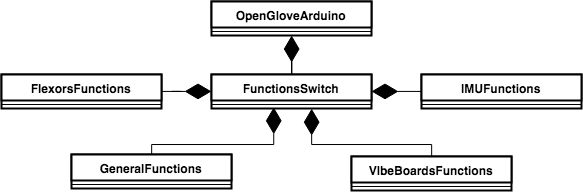
\includegraphics[width=1.0\textwidth]{images/chapter04/OpenGlove-Architecture-Arduino-Software.png} 
    \caption[Estructura del software de control Arduino]{Estructura del software de control Arduino \\Fuente: Elaboración propia (2018)}
    \label{fig:arduino-software-control}
  \end{center}
\end{figure}

%\captionsetup{justification=centering}
%\caption[Descripción de la estructura software de control Arduino]{Descripción estructura del software de control Arduino \\Fuente: Elaboración propia (2018)}
%\label{table:arduino-software-control}

\begin{table}[H]
\centering
\captionsetup{justification=centering}
\caption[Descripción de la estructura software de control Arduino]{Descripción estructura del software de control Arduino \\Fuente: Elaboración propia (2018)}
\label{table:arduino-software-control}
\begin{tabular}{|l|l|l|l|}
\hline
Nombre             & Descripción                                                                                                                                                                                                                                                                                                                                                                                                                                 & Origen                                                    & Estado Actual                                           \\ \hline
OpenGloveArduino   & \begin{tabular}[c]{@{}l@{}}"Contiene el código principal de Arduino,\\ desde el cual se realizan los llamados\\ de las funciones disponibles en\\ FunctionsSwitch.  Algunas de éstas son\\ invocadas solo cuando  hay datos \\ disponibles, mientras que las funciones\\ que requieren un llamado constante como\\ las dedicadas a la lectura de un sensor,\\ son llamadassin necesidad de datos\\ entrantes" (Cerda, 2017).\end{tabular} & \begin{tabular}[c]{@{}l@{}}Cerda\\ (2017)\end{tabular}    & Modificado                                              \\ \hline
FunctionsSwitch    & \begin{tabular}[c]{@{}l@{}}"Se encarga de evaluar e invocar el tipo\\ defunción  solicitada, con el fin de\\ realizar cambios en la  instancia de la\\ biblioteca correspondiente a dicha\\ función"(Cerda, 2017).\end{tabular}                                                                                                                                                                                                           & \begin{tabular}[c]{@{}l@{}}Cerda\\ (2017)\end{tabular}    & \begin{tabular}[c]{@{}l@{}}Sin\\ modificar\end{tabular} \\ \hline
GeneralFunctions   & \begin{tabular}[c]{@{}l@{}}Contiene las funciones generales de\\ Arduino (lecturas/escrituras y\\ digitales/análogas). Se  destaca la función\\ setLoopDelay() para definir el retraso\\ de los ciclos de la placa\\ en milisegundos. Por defecto es 60 ms,\\ por tanto para obtener la mayor velocidad\\ de la placa Arduino, se debe utilizar la\\ función  SetLoopDelay disponible en la\\ API de alto nivel.\end{tabular}               & \begin{tabular}[c]{@{}l@{}}Monsalve\\ (2015)\end{tabular} & \begin{tabular}[c]{@{}l@{}}Sin\\ modificar\end{tabular} \\ \hline
FlexorsFunctions   & \begin{tabular}[c]{@{}l@{}}"Contiene todas las variables y funciones\\ necesarias para representar los flexores \\ del guante y su configuración." (Cerda, 2017).\\ Si se requiere aumentar la cantidad máxima\\ de flexores por placa (10) debe realizarse a\\ nivel del software de control Arduino.\end{tabular}                                                                                                                        & \begin{tabular}[c]{@{}l@{}}Cerda\\ (2017)\end{tabular}    & \begin{tabular}[c]{@{}l@{}}Sin\\ modificar\end{tabular} \\ \hline
VibeBoardFunctions & \begin{tabular}[c]{@{}l@{}}Contiene todas las funciones necesarias para\\ inicializar, activar y desactivar los actuadores.\end{tabular}                                                                                                                                                                                                                                                                                                    & \begin{tabular}[c]{@{}l@{}}Monsalve\\ (2015)\end{tabular} & \begin{tabular}[c]{@{}l@{}}Sin\\ modificar\end{tabular} \\ \hline
ImuFunctions       & \begin{tabular}[c]{@{}l@{}}"Contiene todas las variables y funciones\\ necesarias para el funcionamiento y\\ configuración del sensor de rastreo \\ IMU." (Cerda, 2017).\end{tabular}                                                                                                                                                                                                                                                      & \begin{tabular}[c]{@{}l@{}}Cerda\\ (2017)\end{tabular}    & \begin{tabular}[c]{@{}l@{}}Sin\\ modificar\end{tabular} \\ \hline
\end{tabular}
\end{table}







\subsection{API C\# de bajo nivel}
Para establecer la comunicación entre la API C\# de bajo nivel  y el software de configuración Arduino, fue necesario rehacer la clase Communication, puesto que estaba pensada solamente para un ambiente de escritorio en Windows. Por ello se define una interfaz ICommunication, que define los métodos que deben ser implementados en las diferentes plataformas objetivo. Los métodos de la interfaz son: la obtención de la lista de dispositivos emparejados, la conexión/desconexión de dispositivos y la escritura/lectura del socket Bluetooth creado. La Figura \ref{fig:api-csharp-ll} muestra el diagrama de clases de la API C\# de bajo nivel  desarrollada.  La Tabla \ref{table:api-csharp-ll} contiene la descripción de cada clase que compone el diagrama de clases, su origen y el estado actual de desarrollo.

%Además cuando establecen conexión, esta debe ser mediante la creación de hilos que administren las conexiones Bluetooth, los cuales se deben suscribir al servidor para enviar los mensajes recibidos. En la sección 4.4 se detallan los aspectos de implementación en base a este diseño.

\begin{figure}[H]
  \begin{center} 
   	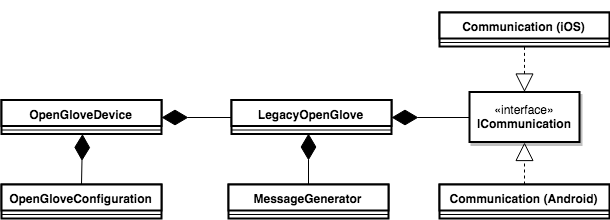
\includegraphics[width=1.0\textwidth]{images/chapter04/OpenGlove-Architecture-API-CSharp-LowLevel.png} 
    \caption[Diagrama de clases API C\# de bajo nivel]{Diagrama de clases API C\# de bajo nivel \\Fuente: Elaboración propia (2018)}
    \label{fig:api-csharp-ll}
  \end{center}
\end{figure}


%\captionsetup{justification=centering}
%\caption[Descripción del diagrama de clases API C\# de bajo nivel]{Descripción del diagrama de clases API C\# de bajo nivel \\Fuente: Elaboración propia (2018)}
%\label{table:api-csharp-ll}


\begin{table}[H]
\centering
\captionsetup{justification=centering}
\caption[Descripción del diagrama de clases API C\# de bajo nivel]{Descripción del diagrama de clases API C\# de bajo nivel \\Fuente: Elaboración propia (2018)}
\label{table:api-csharp-ll}
\begin{tabular}{|l|l|l|l|}
\hline
Nombre                                                             & Descripción                                                                                                                                                                                                                                                                                                                                                                                                                                                                                                                                                    & Origen                                                 & Estado Actual                                                                                           \\ \hline
OpenGloveDevice                                                    & \begin{tabular}[c]{@{}l@{}}Clase que representa un dispositivo OpenGlove,\\ la cual incluye su identificación, configuración y\\ todos los métodos que permiten la comunicación\\ con el software de control Arduino y la inicializa-\\ ción de la configuración en la placa Arduino.\end{tabular}                                                                                                                                                                                                                                                             & Nuevo                                                  & Completado                                                                                              \\ \hline
\begin{tabular}[c]{@{}l@{}}OpenGloveConfi-\\ guration\end{tabular} & \begin{tabular}[c]{@{}l@{}}Representa la configuración global de un\\ dispositivo OpenGlove. Esta incluye la\\ configuración de la placa Arduino, el mapeo de\\ actuadores, el mapeo de flexores y la configuración\\ del IMU. Dicha configuración global puede estar\\ o no inicializada en el dispositivo físico.\end{tabular}                                                                                                                                                                                                                               & Nuevo                                                  & Completado                                                                                              \\ \hline
LegacyOpenGlove                                                    & \begin{tabular}[c]{@{}l@{}}Clase que representa la API C\# de bajo nivel\\ desarrollada por Monsalve (2015) y Cerda (2017),\\ modificada para obtener la versión del software\\ de control Arduino.\end{tabular}                                                                                                                                                                                                                                                                                                                                               & \begin{tabular}[c]{@{}l@{}}Cerda\\ (2017)\end{tabular} & Modificado                                                                                              \\ \hline
MessageGenerator                                                   & \begin{tabular}[c]{@{}l@{}}Clase que permite la generación de mensajes\\ bajo el protocolo establecido por Monsalve (2015)\\ para los actuadores y la extensión realizada por\\ Cerda (2017) para dar soporte a los flexores e\\ IMU. Esta clase fue modificada para obtener\\ la versión del software de control Arduino.\end{tabular}                                                                                                                                                                                                                        & \begin{tabular}[c]{@{}l@{}}Cerda\\ (2017)\end{tabular} & Modificado                                                                                              \\ \hline
ICommunication                                                     & \begin{tabular}[c]{@{}l@{}}Interfaz que contiene la definición de métodos que\\ deben ser implementados para obtener: la lista de\\ dispositivos emparejados, la conexión/desconexión\\ de los mismos y la escritura/lectura de mensajes. \\ Esta interfaz debe ser implementada en cada\\ sistema operativo que desee utilizar OpenGlove,\\ para ello se debe consultar las plataformas\\ soportadas por Xamarin.Forms, este proyecto\\ incluye el soporte para Android.\end{tabular}                                                                         & Nuevo                                                  & Completado                                                                                              \\ \hline
\begin{tabular}[c]{@{}l@{}}Communication\\ (Android)\end{tabular}  & \begin{tabular}[c]{@{}l@{}}Implementación de la interfaz ICommunication\\ en el proyecto Android de Xamarin.Forms. Hace\\ uso de las APIs Bluetooth de Android\\ permitiendo obtener la lista de dispositivos\\ emparejados, la conexión/desconexión de\\ dispositivos y la escritura/lectura del socket\\ Bluetooth creado. Esta clase crea un hilo que\\ administra cada conexión Bluetooth de manera\\ independiente, este hilo permite que otros objetos\\ se suscriban para recibir los mensajes que envie\\ el software de control Arduino.\end{tabular} & Nuevo                                                  & Completado                                                                                              \\ \hline
\begin{tabular}[c]{@{}l@{}}Communication\\ (iOS)\end{tabular}      & \begin{tabular}[c]{@{}l@{}}Implementación de la interfaz\\ ICommunication en el proyecto iOS de\\ Xamarin.Forms. Los métodos de esta clase\\ arrojan la excepción NotImplementedException.\\ Es necesario implementar los métodos de esta\\ clase para dar soporte a OpenGlove en iOS, para\\ ello debe utilizarse un dispositivo físico.\end{tabular}                                                                                                                                                                                                         & Nuevo                                                  & \begin{tabular}[c]{@{}l@{}}Incompleto,\\ se requiere\\ implementar \\ los métodos\\ en iOS\end{tabular} \\ \hline
\end{tabular}
\end{table}




\subsection{APIs alto nivel}
Para permitir la interoperabilidad de OpenGlove, se deben soportar diferentes lenguajes de programación, que son utilizados en el desarrollo móvil de diferentes plataformas, como lo es iOS y Android, por tanto se desarrollaron las APIs C\# y Java como se especifica en el alcance del proyecto. Estas APIs poseen un mismo objetivo, el cual consiste en abstraer la complejidad de conexiones y protocolos de comunicación necesarios, para tener una instancia OpenGlove que permita la interacción en tiempo real con el dispositivo físico. Esto se consigue utilizando el diseño presentado en la Figura \ref{fig:api-csharp-hl} y \ref{fig:api-java-hl}. Se destaca la diferencia en la implementación de WebSocketClient en la clase Communication, debido a las diferencias en el lenguaje de programación y la implementación de las Bibliotecas WebSocket utilizadas en cada API. Esto se debe a que en ambos casos, se busca que la clase Communication sea el acceso a los eventos relacionados con la obtención de mensajes desde el servidor (valores de los flexores, el IMU y el estado de conexión con el dispositivo Bluetooth). La Tabla \ref{table:api-hl-class-diagram-description} contiene la descripción de cada clase que compone el diagrama de clases.


\begin{figure}[H]
  \begin{center} 
   	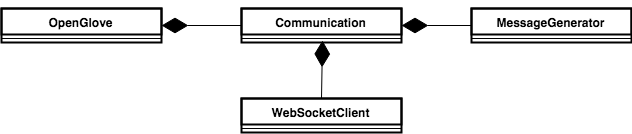
\includegraphics[width=1.0\textwidth]{images/chapter04/OpenGlove-Architecture-API-CSharp-HL.png} 
    \caption[Diagrama de clases API C\# de alto nivel]{Diagrama de clases API C\# de alto nivel \\Fuente: Elaboración propia (2018)}
    \label{fig:api-csharp-hl}
  \end{center}
\end{figure}


Redactando ...

\begin{figure}[H]
  \begin{center} 
   	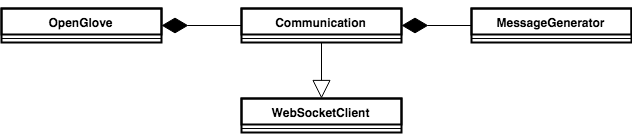
\includegraphics[width=1.0\textwidth]{images/chapter04/OpenGlove-Architecture-API-Java-HL.png} 
    \caption[Diagrama de clases API Java de alto nivel]{Diagrama de clases API Java de alto nivel \\Fuente: Elaboración propia (2018)}
    \label{fig:api-java-hl}
  \end{center}
\end{figure}

%\captionsetup{justification=centering}
%\caption[Descripción del diagrama de clases APIs  de alto nivel]{Descripción del diagrama de clases APIs  de alto nivel \\Fuente: Elaboración propia (2018)}
%\label{table:api-hl-class-diagram-description}

\begin{table}[H]
\centering
\captionsetup{justification=centering}
\caption[Descripción del diagrama de clases APIs  de alto nivel]{Descripción del diagrama de clases APIs  de alto nivel \\Fuente: Elaboración propia (2018)}
\label{table:api-hl-class-diagram-description}
\begin{tabular}{|l|l|}
\hline
Nombre           & Descripción                                                                                                                                                                                                                                                                                                                                                                                                                                                                                                                                                                                                                                                                                                                                                                         \\ \hline
OpenGlove        & \begin{tabular}[c]{@{}l@{}}Clase que representa un dispositivo OpenGlove,\\ la cual incluye su identificación y todos los métodos\\ que permiten la comunicación con el servidor\\ WebSocket, la creación/asignación\\ de la configuración en la instancia OpenGlove\\ del servidor y la inicialización de la  configuración\\  en la placa Arduino.\end{tabular}                                                                                                                                                                                                                                                                                                                                                                                                                   \\ \hline
MessageGenerator & \begin{tabular}[c]{@{}l@{}}Clase que permite la generación de mensajes\\ bajo el protocolo creado por el memorista, para\\ la comunicación Cliente WebSocket y Servidor\\ WebSocket.\end{tabular}                                                                                                                                                                                                                                                                                                                                                                                                                                                                                                                                                                                   \\ \hline
Communication    & \begin{tabular}[c]{@{}l@{}}Clase que permite la comunicación con el Servidor\\ WebSocket, permitiendo el envío/recepción de\\ mensajes bajo el protocolo creado por el memorista.\\ Se utiliza esta clase para la obtención de datos mediante\\ la invocación de métodos, permitiendo crear soluciones\\ en tiempo real suscribiéndose/implementando los\\ siguientes eventos/interfaces:\\ - OnTimeTestServerLatencyActivateActuatorsReceived\\ - OnTimeTestArduinoLatencyActivateActuatorsReceived\\ - OnFlexorValueReceived\\ - OnAccelerometerValuesReceived\\ - OnGyroscopeValuesReceived\\ - OnMagnometerValuesReceived\\ - OnAllIMUValuesReceived\\ - OnBluetoothDeviceConnectionStateChanged\\ - OnWebSocketConnectionStateChangued\\ - OnInfoMessagesReceived\end{tabular} \\ \hline
WebSocketClient  & \begin{tabular}[c]{@{}l@{}}Clase que permite utilizar la API WebSocket,\\ la cual que implementa el protocolo RFC 6455. Se\\ utilizan las bibliotecas disponibles para cada\\ lenguaje de programación.\end{tabular}                                                                                                                                                                                                                                                                                                                                                                                                                                                                                                                                                                \\ \hline
\end{tabular}
\end{table}




\subsection{Aplicación de configuración}
Redactando ... 

\begin{figure}[H]
  \begin{center} 
   	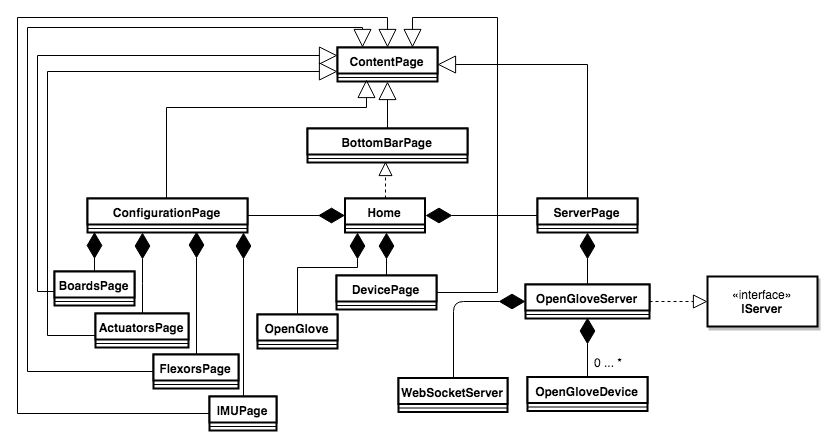
\includegraphics[width=1.0\textwidth]{images/chapter04/OpenGlove-Architecture-Configuration-App.png} 
    \caption[Diagrama de clases aplicación de configuración]{Diagrama de clases aplicación de configuración \\Fuente: Elaboración propia (2018)}
    \label{fig:class-diagram-configuarion-app}
  \end{center}
\end{figure}


%\captionsetup{justification=centering}
%\caption[Descripción del diagrama de clases aplicación de configuración]{Descripción del diagrama de clases aplicación de configuración \\Fuente: Elaboración propia (2018)}
%\label{table:class-diagram-configuarion-app}\\


% Please add the following required packages to your document preamble:
% \usepackage{longtable}
% Note: It may be necessary to compile the document several times to get a multi-page table to line up properly
\begin{longtable}[c]{|l|l|}
\captionsetup{justification=centering}
\caption[Descripción del diagrama de clases aplicación de configuración]{Descripción del diagrama de clases aplicación de configuración \\Fuente: Elaboración propia (2018)}
\label{table:class-diagram-configuarion-app}\\
\hline
Nombre            & Descripción                                                                                                                                                                                                                                                                                                                                                                                                                                                                                                       \\ \hline
\endfirsthead
%
\endhead
%
ContentPage       & \begin{tabular}[c]{@{}l@{}}Xamarin.Forms.ContentPage es una clase y un elemento visual\\ que hereda de la clase base Page en Xamarin.Forms. Otras\\ clases derivadas de Page son MasterDetailPage, NavigationPage,\\ TabbedPage, TemplatedPage y CarrouselPage.\end{tabular}                                                                                                                                                                                                                                      \\ \hline
BottomBarPage     & \begin{tabular}[c]{@{}l@{}}BottomBar.XamarinForms.BottomBarPage es una clase que\\ implementa la  representación visual de la barra inferior en iOS\\ y Android. Permite agregar Pages para representarlos como\\ botones inferiores de navegación.\end{tabular}                                                                                                                                                                                                                                                  \\ \hline
Home              & \begin{tabular}[c]{@{}l@{}}Clase que hereda de BottomBarPage (biblioteca de terceros).\\ Esta clase se instancia como primer Page del NavigationPage,\\ esto permite la navegación jerárquica en la aplicación. La\\ clase NavigationPage implementa la navegación como una\\ lista LIFO (last-in, first-out) de objetos Page.\end{tabular}                                                                                                                                                                       \\ \hline
ConfigurationPage & \begin{tabular}[c]{@{}l@{}}Clase que contiene el menú de acceso a las diferentes\\ interfaces gráficas que permiten la actualización de\\ los actuadores, los flexores e IMU. Permite la creación,\\ lectura, actualización y eliminación (CRUD) de\\ configuraciones globales de OpenGlove.\end{tabular}                                                                                                                                                                                                         \\ \hline
BoardsPage        & \begin{tabular}[c]{@{}l@{}}Clase que provee la interfaz gráfica para modificar la\\ configuración de la placa Arduino, es decir, la configuración\\ de los pines de la placa, cantidad, tipo de señal (análoga/digital),\\ tipo de componente asociado (VibeBoards, Flexores) y \\ polaridad del pin (positiva/negativa). Permite la creación de\\ nuevos modelos de placas, especificando: nombre de la\\ placa, cantidad de pines digitales, cantidad de pines análogos y\\ el primer pin análogo.\end{tabular} \\ \hline
ActuatorsPage     & \begin{tabular}[c]{@{}l@{}}Clase que provee la interfaz gráfica para modificar la configuración\\ de los actuadores, es decir, el mapeo región-actuador, el rango de regiones\\ disponible es dinámica según se requiera, permitiendo cambiar\\ la imagen referencial del mapeo utilizar. Además permite testear\\ los actuadores, especificando la intensidad.\end{tabular}                                                                                                                                      \\ \hline
FlexorPage        & \begin{tabular}[c]{@{}l@{}}Clase que provee la interfaz gráfica para modificar la configuración de los\\ flexores, es decir, el mapeo region-flexor, el rango de regiones\\ disponible es dinámica según se requiera, esto permite cambiar\\ la imagen referencial del mapeo a utilizar. Además permite testear los\\ flexores, mostrando el valor leído desde la placa Arduino con el Threshold\\ permite asignado.\end{tabular}                                                                                 \\ \hline
IMUPage           & \begin{tabular}[c]{@{}l@{}}Clase que provee la interfaz gráfica para modificar la configuración del\\ IMU (SparkFun LSM9DS1). Además permite testear el IMU, mostrando\\ los valores leídos desde la placa Arduino según se especifique.\end{tabular}                                                                                                                                                                                                                                                             \\ \hline
DevicePage        & \begin{tabular}[c]{@{}l@{}}Clase que muestra todos los dispositivos emparejados, permitiendo\\ asignar la configuración global OpenGlove que se quiera inicializar en la\\ placa Arduino.\end{tabular}                                                                                                                                                                                                                                                                                                            \\ \hline
ServerPage        & \begin{tabular}[c]{@{}l@{}}Clase que provee la interfaz gráfica para modificar la configuración del \\ servidor, permitiendo la modificación de la dirección del servidor\\ WebSocket, además del encendido y apagado del mismo.\end{tabular}                                                                                                                                                                                                                                                                     \\ \hline
IServer           & Interfaz que define los métodos Start, Stop y ConfigureServer.                                                                                                                                                                                                                                                                                                                                                                                                                                                    \\ \hline
OpenGloveServer   & \begin{tabular}[c]{@{}l@{}}Clase que provee el acceso a todas las funcionalidades de la aplicación de\\ configuración. Posee todas las instancias de OpenGloveDevice, de los\\ clientes WebSocket conectados y recibe los mensajes de los hilos que\\ administran las conexiones con los dispositivos Bluetooth.\end{tabular}                                                                                                                                                                                     \\ \hline
WebSocketServer   & \begin{tabular}[c]{@{}l@{}}Clase que permite utilizar la API WebSocket, la cual implementa el \\ protocolo RFC 6455. Se utiliza la biblioteca Fleck.\end{tabular}                                                                                                                                                                                                                                                                                                                                                 \\ \hline
OpenGlove         & Clase de alto nivel de OpenGlove ya descrita en la Tabla 4.2                                                                                                                                                                                                                                                                                                                                                                                                                                                      \\ \hline
OpenGloveDevice   & Clase de bajo nivel de OpenGlove ya descrita en la Tabla 4.3                                                                                                                                                                                                                                                                                                                                                                                                                                                      \\ \hline
\end{longtable}
    
    
    
